\section{Results}\label{sec:results}
We now discuss our two aims: more effective learning and a more stable environment.

\subsection{Sample Entropy}
\subsubsection{Observing Lower Sample Entropy}
As the primary objective of a surprise minimization technique is to, in fact,  minimize surprise, it is natural to determine whether SMiRL does so.

We first quantify the degree to which the environment is more or less entropic when under the influence of an agent employing SMiRL. Since we assume each variable in our sample space is normally distributed in a given timeframe, we can compute its entropy as $ H = \frac{1}{2} \ln (2 \pi e \sigma^2)$. For each step, we compute the sample variance of the last 100 steps and use this to compute a sample entropy, shown in \textbf{Figure \ref{fig:sample_entropy}}. 

While both agents do reduce the sample entropy over time, the SMiRL + PPO agent does so earlier than the baseline PPO agent, with significant decay beginning around step 50k v.s. step 100k. 
The SMiRL + PPO implementation exhibits lower sample entropy for all iterations compared to baseline PPO, and hence energy usage over the course of the simulation is more consistent when using SMiRL.

Additionally, the SMiRL + PPO agent converges towards a policy which generates a more stable final environment than the baseline PPO agent. %TODO: Explain jumps in entropy for baseline agent
The SMiRL + PPO agent's behaviour confirms our hypothesis that the stability of our environment is superior to our baseline PPO agent by incentivizing the RL agent to revisit familiar states. 
We also note that the both agents continue to explore changes to their policies after convergence, however the SMiRL + PPO maintains a lower sample entropy in late timesteps. Hence, the SMiRL + PPO agent explores in ways that maintain a more stable environment, while the PPO agent's exploration results in more unstable energy usage.

In this sense, the addition of the SMiRL reward can allow an agent to strike a balance between exploration and stability. 
\begin{figure}
    \centering
    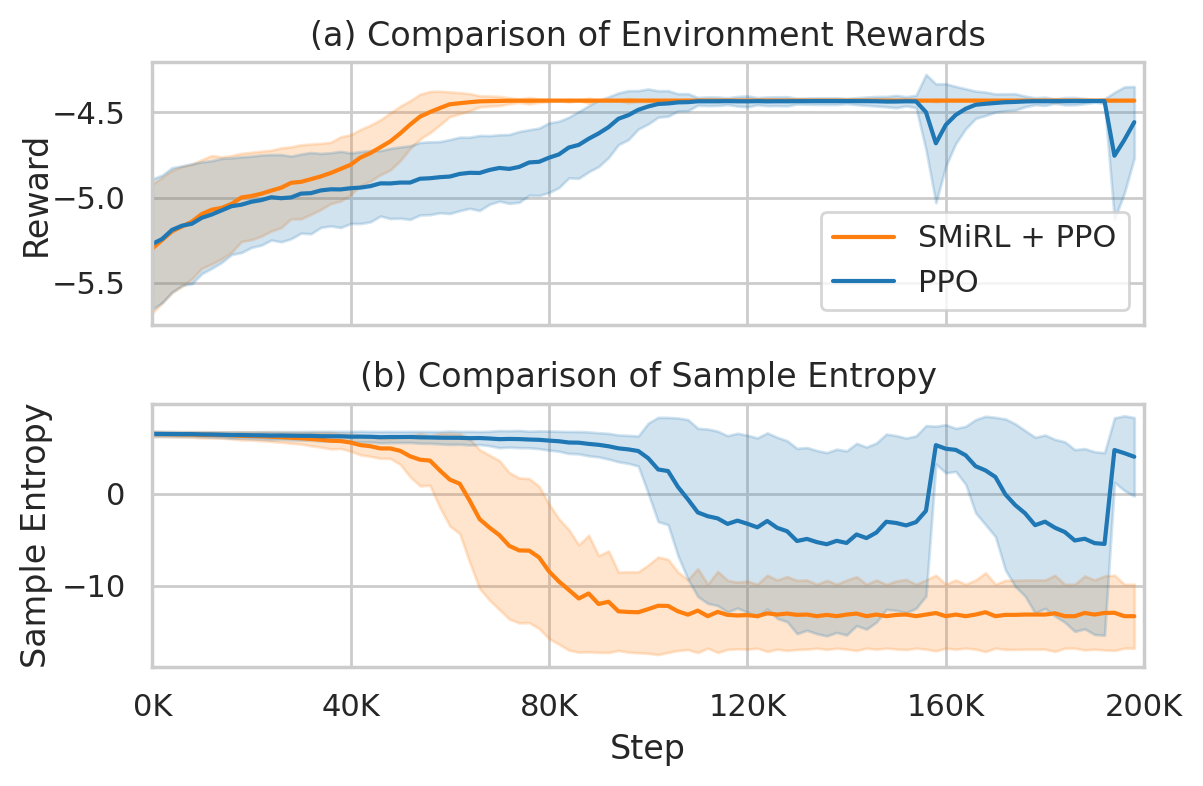
\includegraphics[width=\linewidth]{graphics/combined_ent_rew.png}
    \caption{A comparison between the PPO + SMiRL agent and the baseline PPO agents' (a) rewards and (b) sample entropies over training steps. Shaded regions are one standard deviation of observations binned to every 100 steps.}
    \label{fig:sample_entropy}
\end{figure}

\subsection{Improved Learning with SMiRL (Compared to Baseline PPO)}
While environment stability is important, it is essenital that the agent still encorages efficient energy usage. We also wish to understand whether the SMiRL reward models our assumption of predictability in our system by improved learning speed.

\subsubsection{Faster Learning and Consistent Outcomes}\label{sec:RL_learning}
We observe that our SMiRL + PPO implementation induces significantly faster learning and convergence to an equally optimal policy, with the same reward. 
As shown by Figure \ref{fig:sample_entropy}(a), both agents maintain similar rewards up until step \textasciitilde 30k, after which the SMiRL + PPO agent begins to achieve, on average, a higher reward.
The SMiRL + PPO implementation converges in roughly half the time as the baseline PPO agent (step \textasciitilde 50k v.s. step \textasciitilde 110k). The reward in the environment around step \textasciitilde 60k whereas the PPO baseline does not 
converge to the maximum reward in the environment until step \textasciitilde 110k. 
Our results support our hypothesis that an auxilary SMiRL reward improves learning speed. 

Note that we compare the energy rewards ($r_\text{energy}$) here directly and not the combined reward which includes the SMiRL reward and weight. This demonstrates the influence of the SMiRL reward on the energy reward, which describes the overall effectiveness of our agent. Hence the inclusion of the SMiRL reward results in improved learning speed of our agent in the task it is given. 
\begin{figure}
    \centering
    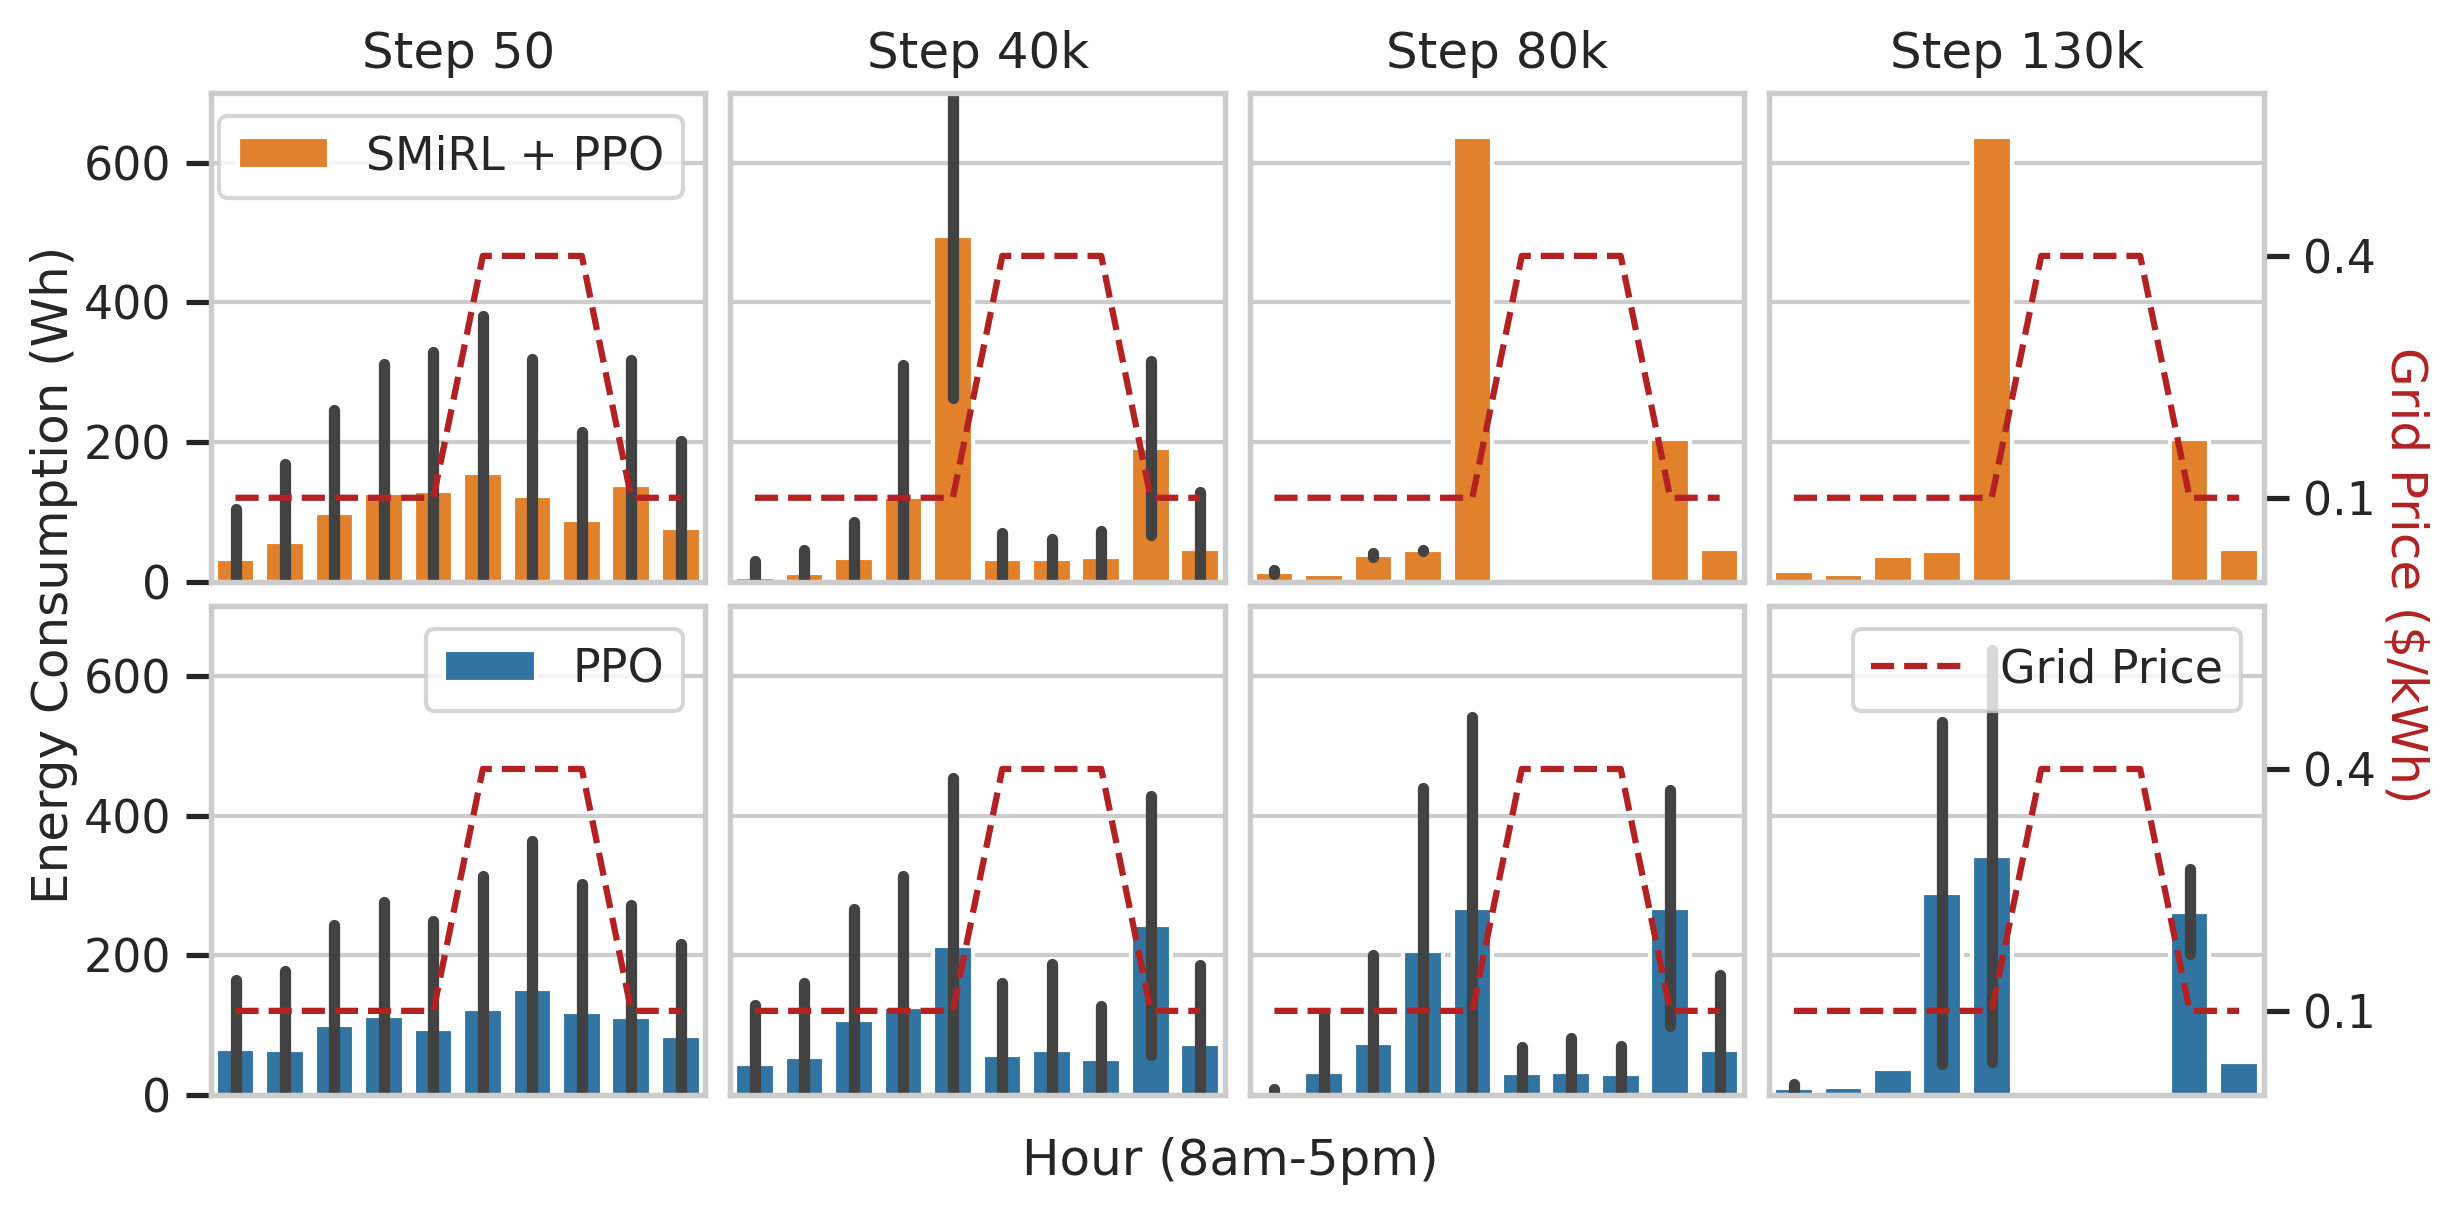
\includegraphics[width=\linewidth]{graphics/mmmmfirebrick.png}
    \caption{Energy consumption with the PPO and SMiRL + PPO agent at steps 10k, 40k, 80k, and 130k compared to the grid price. Please see section \ref{sec:discussion} for a brief note on the seemingly adverse behavior in the SMiRL+PPO.}
    \label{fig:observations}
\end{figure}

Faster convergence is demonstrated by \ref{fig:observations}, where energy consumption is shown at different steps in the environment.
The grid price signal the agent recieves is shown. We observe that, for both the PPO and SMiRL + PPO agent, the price signal  effectively shifts people's energy consumption away from times when the grid price is higher.
By step 40k, however, the SMiRL + PPO agent has already begun to greatly reduce consumption during peak, and people have shifted it towards just before that peak.
By step 80k, the SMiRL + PPO agent has completely diminished any energy usage during the peak pricing, while the PPO agent only does so by step \textasciitilde 120k (when its reward converges).



\subsubsection{Optimal SMiRL Weights}
We note that while an appropriate SMiRL weight provides significant improvement in learning speed
and sample entropy, an inadequate SMiRL weight can lead to poor learning that converges to a suboptimal result, and may not outperform a baseline PPO. 

Specifically, we found SMiRL weights of $ \alpha = 0.25$ and higher performed worse than baseline PPO. 
In fact, we find that they converge to a suboptimal reward in the environment, hinting that too much surprise minimization might hinder exploration. 

For much lower SMiRL weights such as $ \alpha = 0.01 $, we do not see any 
significant benefits when compared to baseline PPO; there isn't enough 
weight on the SMiRL reward to have a meaningful impact. 

\subsubsection{Sample Entropy and Environment Reward Curves}
When comparing the sample entropy and reward curves in \textbf{Figure \ref{fig:sample_entropy}} 
we see that beginning at steps \textasciitilde 50k, the SMiRL + PPO agent's observed 
sample entropy drops significantly below that of the baseline PPO agent. 
This correlates closely at \textasciitilde 50k steps where the PPO + SMiRL implementation begins to experience significantly greater rewards than baseline PPO. 
Lastly, we observe that at \textasciitilde 110k steps, both agents have observed a drop in sample entropy, and their environment rewards converge.
This correlation between entropy and reward may support our hypothesis that aiming for a stable environment via surprise minimization can help the agent learn faster.

% TODO: sentence or two talking about abstraction of system 
